\documentclass[10pt]{book}
\usepackage{graphicx}
\usepackage{subfig} % make it possible to include more than one captioned figure/table in a single float
\usepackage[utf8]{inputenc}
\usepackage{hyperref}
\usepackage[intlimits]{amsmath}
\usepackage{amssymb}
\usepackage{float}
\setlength{\oddsidemargin}{15.5pt} 
\setlength{\evensidemargin}{15.5pt}
\pretolerance=2000
\tolerance=3000
\renewcommand{\figurename}{Figura}
\renewcommand{\chaptername}{Cap\'{i}tulo}
\renewcommand{\contentsname}{\'{I}ndice}
\renewcommand{\tablename}{Tabla}
\renewcommand{\bibname}{Bibliograf\'{i}a}
\renewcommand{\appendixname}{Ap\'endices}


\usepackage{geometry}
 \geometry{
 a4paper,
 left=5mm,
 right=5mm,
 top=5mm,
 bottom=5mm,
 }

\begin{document}

\begin{figure}[H]
 \centering
 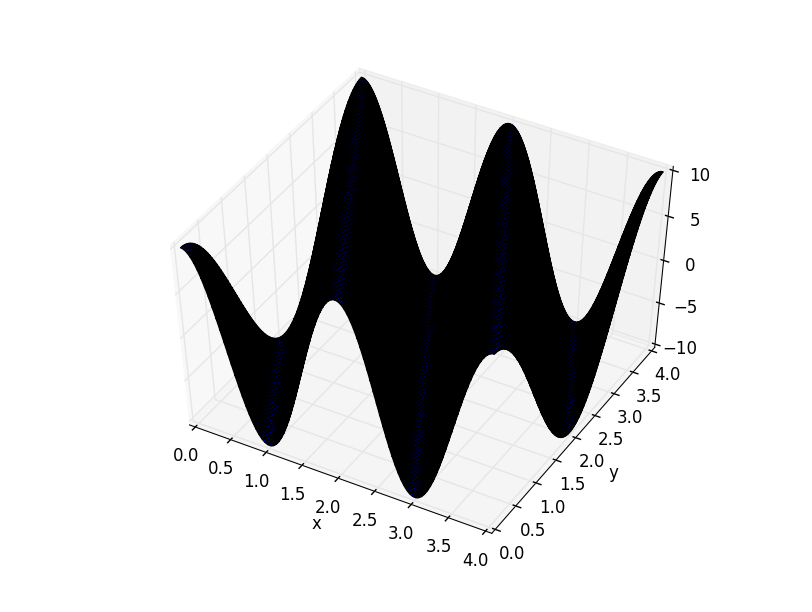
\includegraphics[scale=0.8]{1.png}
\end{figure}

\begin{figure}[H]
 \centering
 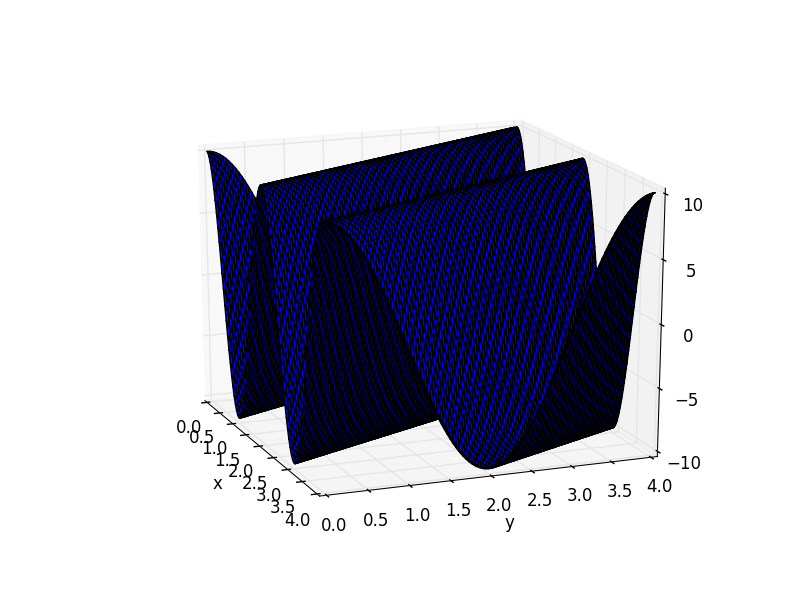
\includegraphics[scale=0.8]{2.png}
\end{figure}

\begin{figure}[H]
 \centering
 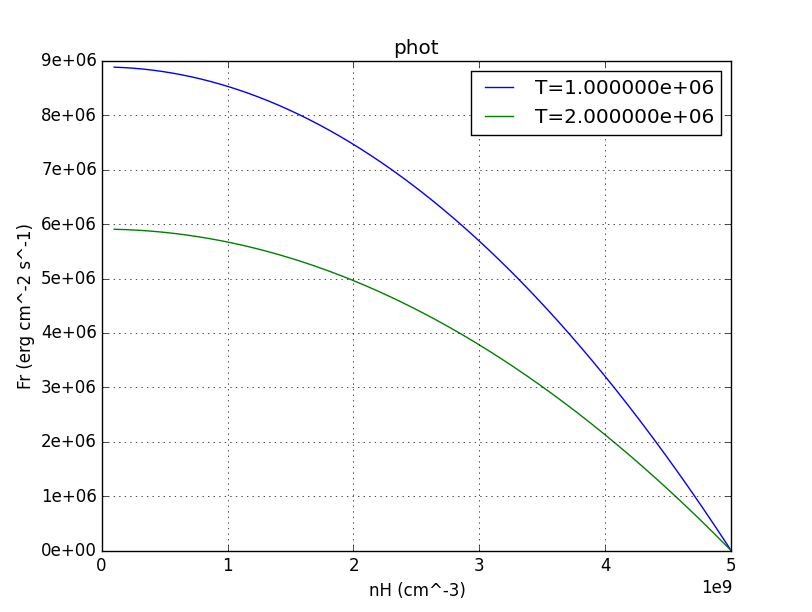
\includegraphics[scale=0.6]{Frphot.png}
 \caption{\emph{Fr using Lambda Ph}}
\end{figure}

\begin{figure}[H]
 \centering
 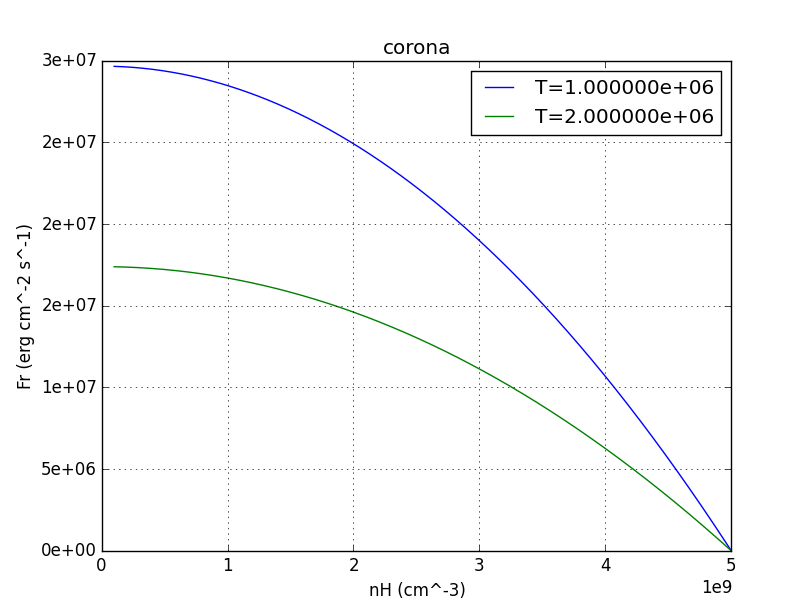
\includegraphics[scale=0.6]{Frcorona.png}
 \caption{\emph{Fr using Lambda Corona}}
\end{figure}

\begin{verbatim}
corona
T=1.000000e+06
Lr(nH = 4.991669e+09) = 9.878355e+04 ; in model: nH = 4.917633e+09 at z = 1.421240e+00 Mm
Lr(nH = 4.999020e+09) = 1.163014e+04 ; in model: nH = 4.917633e+09 at z = 1.421240e+00 Mm
Lr(nH = 4.559446e+09) = 4.997929e+06 ; in model: nH = 4.548157e+09 at z = 1.440790e+00 Mm
T=2.000000e+06
Lr(nH = 4.985789e+09) = 9.873613e+04 ; in model: nH = 4.917633e+09 at z = 1.421240e+00 Mm
Lr(nH = 4.998530e+09) = 1.022712e+04 ; in model: nH = 4.917633e+09 at z = 1.421240e+00 Mm
Lr(nH = 4.220822e+09) = 4.998763e+06 ; in model: nH = 4.226348e+09 at z = 1.460330e+00 Mm
phot
T=1.000000e+06
Lr(nH = 4.971577e+09) = 1.007338e+05 ; in model: nH = 4.917633e+09 at z = 1.421240e+00 Mm
Lr(nH = 4.997060e+09) = 1.044737e+04 ; in model: nH = 4.917633e+09 at z = 1.421240e+00 Mm
Lr(nH = 3.306391e+09) = 4.999994e+06 ; in model: nH = 3.245860e+09 at z = 1.538510e+00 Mm
T=2.000000e+06
Lr(nH = 4.957366e+09) = 1.003062e+05 ; in model: nH = 4.917633e+09 at z = 1.421240e+00 Mm
Lr(nH = 4.995590e+09) = 1.041634e+04 ; in model: nH = 4.917633e+09 at z = 1.421240e+00 Mm
Lr(nH = 1.959246e+09) = 4.999980e+06 ; in model: nH = 1.923238e+09 at z = 1.714420e+00 Mm

WITH INTERPOLATION for findind nH from Lr:

corona
T=1.000000e+06
Lr(nH = 4.991566e+09) = 1.000000e+05 ; in model: nH = 4.917633e+09 at z = 1.421240e+00 Mm
Lr(nH = 4.999157e+09) = 1.000000e+04 ; in model: nH = 4.917633e+09 at z = 1.421240e+00 Mm
Lr(nH = 4.559255e+09) = 5.000000e+06 ; in model: nH = 4.548157e+09 at z = 1.440790e+00 Mm
T=2.000000e+06
Lr(nH = 4.985606e+09) = 1.000000e+05 ; in model: nH = 4.917633e+09 at z = 1.421240e+00 Mm
Lr(nH = 4.998563e+09) = 1.000000e+04 ; in model: nH = 4.917633e+09 at z = 1.421240e+00 Mm
Lr(nH = 4.220611e+09) = 5.000000e+06 ; in model: nH = 4.226348e+09 at z = 1.460330e+00 Mm
phot
T=1.000000e+06
Lr(nH = 4.971785e+09) = 1.000000e+05 ; in model: nH = 4.917633e+09 at z = 1.421240e+00 Mm
Lr(nH = 4.997186e+09) = 1.000000e+04 ; in model: nH = 4.917633e+09 at z = 1.421240e+00 Mm
Lr(nH = 3.306388e+09) = 5.000000e+06 ; in model: nH = 3.245860e+09 at z = 1.538510e+00 Mm
T=2.000000e+06
Lr(nH = 4.957496e+09) = 1.000000e+05 ; in model: nH = 4.917633e+09 at z = 1.421240e+00 Mm
Lr(nH = 4.995766e+09) = 1.000000e+04 ; in model: nH = 4.917633e+09 at z = 1.421240e+00 Mm
Lr(nH = 1.959224e+09) = 5.000000e+06 ; in model: nH = 1.923238e+09 at z = 1.714420e+00 Mm




\end{verbatim}



\end{document}
